\chapter{Introdução}\label{introducao}
% determinacao da potencia sonora
Várias técnicas de controle de ruído foram desenvolvidas nesses últimos tempos visando oferecer ao ouvido humano um ambiente agradável, principalmente em ambientes de salas nas quais aspecto reverberante é bastante evidente.

Com esse determinado fim, o uso de materiais de absorção de ondas sonoras é amplamente utilizado. Esses materiais, normalmente porosos, ficam nas extremidades de uma sala reverberante amortecendo e dissipando em forma de energia térmica o som. Em vista desse aspecto todo material que visa esse objetivo possui um coeficiente de absorção sonora e o mesmo é levado em consideração para o controle de ruído numa sala por exemplo.

Em vista do que foi exposto, esse trabalho tem como objetivo analisar o coeficiente de absorção sonora de uma amostra de um material poroso através da câmara de reverberação. Para isso, utilizou-se
como base a norma ISO 354:2003, que estabelece os procedimentos que devem ser feitos para
determinar tal parâmetro em uma câmara reverberante

\chapter{Fundamentação Teórica}\label{fundamentacao}
% Som
Em vista do que se expõe em \cite{bistafa}, o som é a aceleração de partículas de ar que se chocam, transformando a pressão estática do ar numa pressão oscilatória. Essa pressão oscilatória entre em contato com os ouvidos do ouvinte fazendo com que essa variação de pressão seja percebida e escutada. Essa variação de pressão que oscila é escutada pelo ser humano a partir da magnitude de pressão de $2\cdot10^{-5}$ $Pa$. Qualquer pertubação de pressão que se encaixa nessas condições é denominada som e as pertubações indesejáveis são denominadas de ruído sonoro.

Para se mensurar o nível de pressão sonora deve-se comparar	o valor $rms$ da pressão coletada pela pressão de referência ($2\cdot10^{-5}$ $Pa$), usando a operação de divisão. Como a magnitude dessa divisão é muita alta, a variação das pressões audíveis é de ordem muito alta fazendo assim que se transforme esse valor numa medida logarítmica e multiplicado por 10. A expressão matemática resultante desse processo é 
\begin{equation}
  NPS  = 10 . log_10(p_{rms}^{2}/(2\cdot10^{-5})^{2}).
\end{equation}
Tal que $NPS$ é o nível de pressão sonora e $p_{rms}$ é o $rms$ da pressão coletada.
% pressao sonora

% potencia
De acordo com \cite{potencia}, a potência sonora é uma grandeza física que diz respeito à energia acústica total emitida por uma determinada fonte sonora. Dessa forma, a potência sonora depende apenas da própria fonte e independe das características do meio, fazendo com que esse tipo de grandeza física se qualifique como satisfatório para caracterizar uma fonte sonora. Em vista disso a potência sonora é dada pela equação
\begin{equation}
W = I_{max}S.
\label{eq.potencia}
\end{equation}
Tal que $W$ é a potência sonora, $I_{max}$ intensidade sonora máxima e $S$ é a área. Como a intensidade sonora máxima ($I_{max}$) se relaciona com a impedância característica do meio ($\rho . c$) de tal forma que a expressão matemática de denota como \begin{equation}
I_{max}=\frac{p_{rms}^{2}}{\rho_{0} . c}.
\label{eq.intensidade}
\end{equation}
Dessa forma, dividindo por uma potência de referência $W_{o}= \frac{p_{o}^{2}}{\rho c}S $ a equação da potência pode ser caracterizada por
 \begin{equation}
	\frac{W}{W_{o}}=\frac{p_{rms}^{2}}{p_{o}^{2}}\frac{S}{S_{o}}.
\label{eq.relpotencia}
\end{equation}
Aplicando a operação logarítmica na equação \ref{eq.relpotencia} o resultado final do cálculo da potência é
\begin{equation}
	NWS = NPS + 10 . log_{10}\left(\frac{S}{S_{o}}\right).
\end{equation}

% calculo potencia anecoicaa

Para o cálculo dos coeficientes de absorção sonora de um material usando um tubo de impedância, é preciso considerar duas ondas sonoras no duto: ondas de reflexão e ondas de incidência, que trabalham abaixo da frequência de corte. Ambas respectivamente podem ser calculadas através das equações \ref{eq.pressao_incidente} e \ref{eq.pressao_refletida}.

\begin{equation}
p_{i}=\widehat{p}_{i}e^{\textbf{j}kx}\;,
\label{eq.pressao_incidente}
\end{equation}
\begin{equation}
p_{r}=\widehat{p}_{r}e^{-\textbf{j}kx}\;,
\label{eq.pressao_refletida}
\end{equation}
\noindent{Dos quais $\widehat{p}_{i}$ e $\widehat{p}_{r}$ são as magnitudes de $p_{i}$ e $p_{r}$ em um plano de referência ($x=0$). Portanto a pressão sonora total é caracterizada pela soma entre a pressão sonora incidente e a pressão sonora refletida.}

\begin{equation}
p= \widehat{p}_{i}e^{\textbf{j}kx} + \widehat{p}_{r}e^{-\textbf{j}kx}
\end{equation}

O sistema possui duas incógnitas, as amplitudes das pressões complexas, tanto incidente como refletida. Portanto, para solucionar esse sistema de equações é necessário obter dois dados de pressão sonora.

\begin{equation}
p_{1}= \widehat{p}_{i}e^{\textbf{j}kx_{1}} + \widehat{p}_{r}e^{-\textbf{j}kx_{1}}
\end{equation}

\begin{equation}
p_{2}= \widehat{p}_{i}e^{\textbf{j}kx_{2}} + \widehat{p}_{r}e^{-\textbf{j}kx_{2}}
\end{equation}

Pode-se ainda relacionar esses dois dados de pressão sonora através de uma função de transferência, definida pela equação \ref{eq.funcao_transferencia}.
\begin{equation}
H_{12}=\frac{p_{2}}{p_{1}}
\label{eq.funcao_transferencia}
\end{equation}

Para se obter maior precisão na função de transferência, é necessário fazer duas medições: uma com os microfones numa dada posição padrão e outra com eles trocados de posição. Desse modo pode-se retirar a diferença de fase entre os dois microfones aplicando a equação \ref{eq.funcao_transferencia_correcao}.
\begin{equation}
	H_{corrigida} = \frac{\sqrt{H_{posicao_1}}}{\sqrt{H_{posicao_2}}}
\label{eq.funcao_transferencia_correcao}
\end{equation} 

De forma análoga, obtêm-se funções de transferências para as pressões sonoras incidentes e para as pressões sonoras refletidas, conforme as Equações \ref{eq.funcao_transferencia_i} e \ref{eq.funcao_transferencia_r}, respectivamente.

\begin{equation}
H_{I} = \frac{p_{i_{2}}}{p_{i_{1}}}=e^{-\textbf{j}k(x_{1}-x_{2})}=e^{-\textbf{j}ks}
\label{eq.funcao_transferencia_i}
\end{equation} 

\begin{equation}
H_{R} = \frac{p_{r_{2}}}{p_{r_{1}}}=e^{-\textbf{j}k(x_{1}-x_{2})}=e^{\textbf{j}ks}
\label{eq.funcao_transferencia_r}
\end{equation}

\noindent{onde $s$ é a distância entre os dois transdutores utilizados para medir a pressão sonora no duto.}

Através dessas funções de transferências pode-se se obter o fator de reflexão sonora $r$ em um plano de referência ($x=0$), conforme a equação \ref{eq.fator_reflexao}.

\begin{equation}
r=\frac{H_{12}-H_{I}}{H_{R}-H_{12}}e^{2\textbf{j}kl}\;,
\label{eq.fator_reflexao}
\end{equation}

Por fim, o cálculo do coeficiente de absorção sonora $\alpha$ para uma onda de incidência normal a superfície do material pode ser calculado através da equação \ref{eq.absorcao}.
\begin{equation}
\alpha=1-|r|^{2}
\label{eq.absorcao}
\end{equation} 

\chapter{Experimento e Equipamentos}\label{descricao}

O método baseia-se na norma ISO 10534-2:1998, que descreve a utilização de dois microfones em um duto de superfícies rígidas, denominado tubo de impedância, de posse de um analisador digital de sinais é possível determinar o coeficiente de absorção sonora de materiais para uma onda sonora de incidência normal, impedâncias superficiais e admitâncias de materiais absorventes.  

Em uma das terminações do tubo está posicionada a fonte sonora, e na outra terminação a amostra do material a ser analisado. Nesse método as ondas planas são geradas por uma fonte de ruído, e a decomposição entre a onda incidente e refletida é feita através da medição com dois transdutores fixos é uma determinada posição, de modo que é feita a aquisição da função de transferência entre os microfones. A Figura \ref{fig.equipamento} e a Tabela \ref{tab.bancada} exibem e listam, respectivamente, como é feita a montagem da bancada para a determinação do coeficiente de absorção sonora de um material em um tubo de impedância.

\begin{figure}[h]
\centering
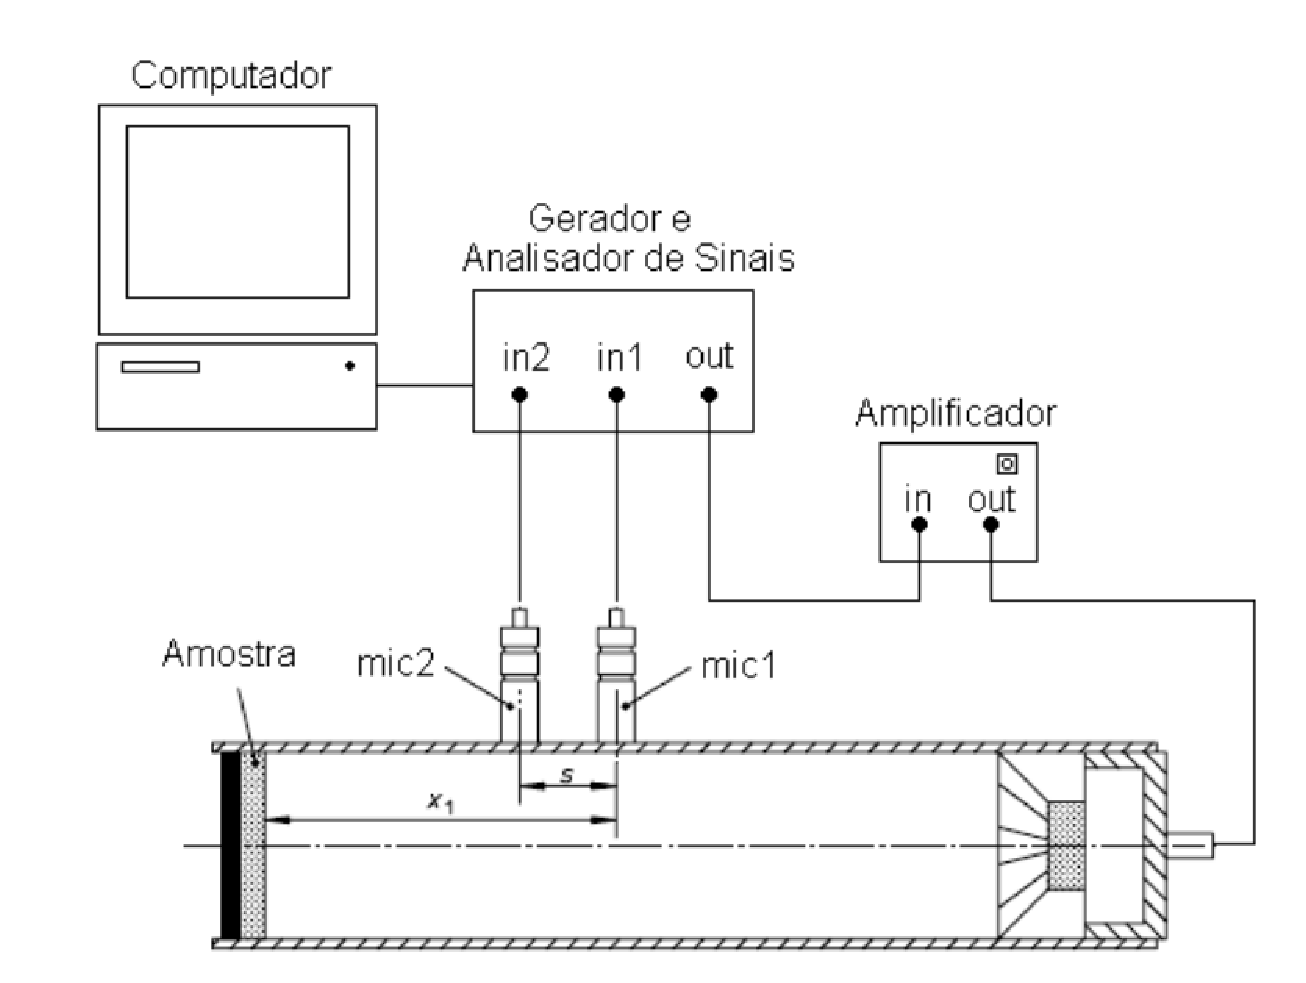
\includegraphics[scale=0.45]{figs/bancada.eps}
\caption{Equipamentos utilizados para a medição a determinação do coeficiente de absorção sonora de um material em um tubo de impedância. Fonte \cite{mareze2013analise}}
\label{fig.equipamento}
\end{figure}  

\begin{table}[h]
\centering
\caption{Equipamentos utilizados na medição.}
\label{tab.bancada}
\begin{tabular}{l|l}
Item               & Descrição do Equipamento                                 \\ \hline
1                  & Analisador de sinais B\&K Pulse             \\
2                  & Computador com o programa Pulse LabShop       \\
3                  & Amplificador B\&K 2619\                    \\
4                  & Microfones de 1/2'' modelo B\&K 4189         \\
5                  & Calibrador 200 Larson Davids \\
                                                        
\end{tabular}
\end{table}

O material poroso analisado foi uma lã de vidro produzido pela empresa \textit{Rockfibras}, conforme a Figura \ref{fig.rockfibras}. Primeiramente foi feita a medição da função de transferência entre os microfones sem a presença do material poroso com o intuito de verificar se há absorção sonora nas superfícies do tubo, visto que as superfícies não são idealmente rígidas.
\begin{figure}[h]
\centering
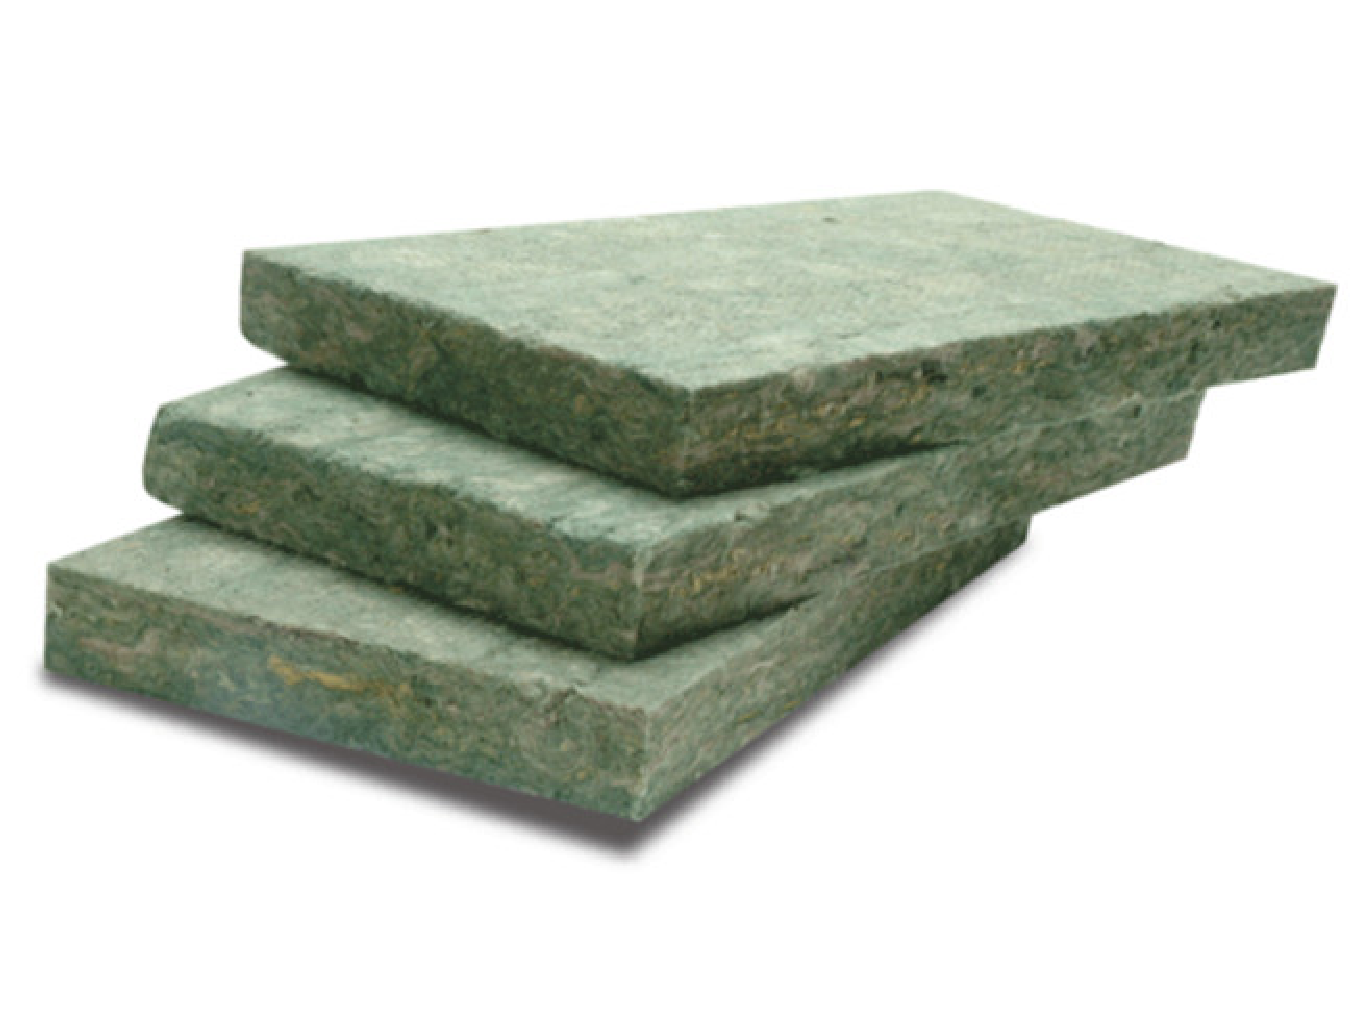
\includegraphics[scale=0.35]{figs/rockfibras.eps}
\caption{Lã de rocha utilizada para o ensaio.}
\label{fig.rockfibras}
\end{figure}



Posteriormente foi recortada três (3) amostras de lã de vidro do mesmo material, porém com espessuras $h$ ligeiramente diferentes, exibidas na Tabela \ref{tab.espessuras}. O objetivo foi medir separadamente cada uma das amostras e verificar se o coeficiente de absorção sonora teve resultados semelhantes para os três ensaios.

\begin{table}[h]
\centering
\caption{Espessuras das amostras ensaiadas}
\label{tab.espessuras}
\begin{tabular}{l|l}
Item                       & Espessura (mm)      \\ \hline
Amostra 1                  & 25.2                  \\
Amostra 2                  & 25.8               \\
Amostra 3                  & 25.6                  \\
\end{tabular}
\end{table}

Para cada medição foi extraído como resposta as funções de transferências $H_{12}$ através de um \textit{template} programado no software Pulse LabShop. Como já foi discutido anteriormente, a partir das funções de transferência entre os microfones é possível extrair o coeficiente de absorção sonora por incidência direta de um material.

Outra técnica utilizada nesse trabalho foi o intercâmbio entre as posições dos microfones, essa técnica é utilizada para corrigir a diferença de fase entre os microfones. Para tanto, calcula-se uma nova função de transferência $H_{12}^{''}$
\begin{equation}
	H_{12}^{'} = \frac{p_\textbf{mic1}}{p_\textbf{mic2}}\;,
\hspace{1.5 cm} \textbf{e} \hspace{1.5 cm} H_{12}^{''} = \frac{p_\textbf{mic2}}{p_\textbf{mic1}}\;,  	
\end{equation}
\noindent{onde $H_{12}^{'}$ é a função de transferência sem intercâmbio de microfones e $H_{12}^{''}$ é a função de transferências com intercâmbio de microfones.}

Por fim, a Figura \ref{fig.experimento} é exposta para exibir a bancada de onde foi extraída as funções de transferência entre os microfones para a determinação do coeficiente de absorção $\alpha$ do material poroso.

\begin{figure}[h]
\centering
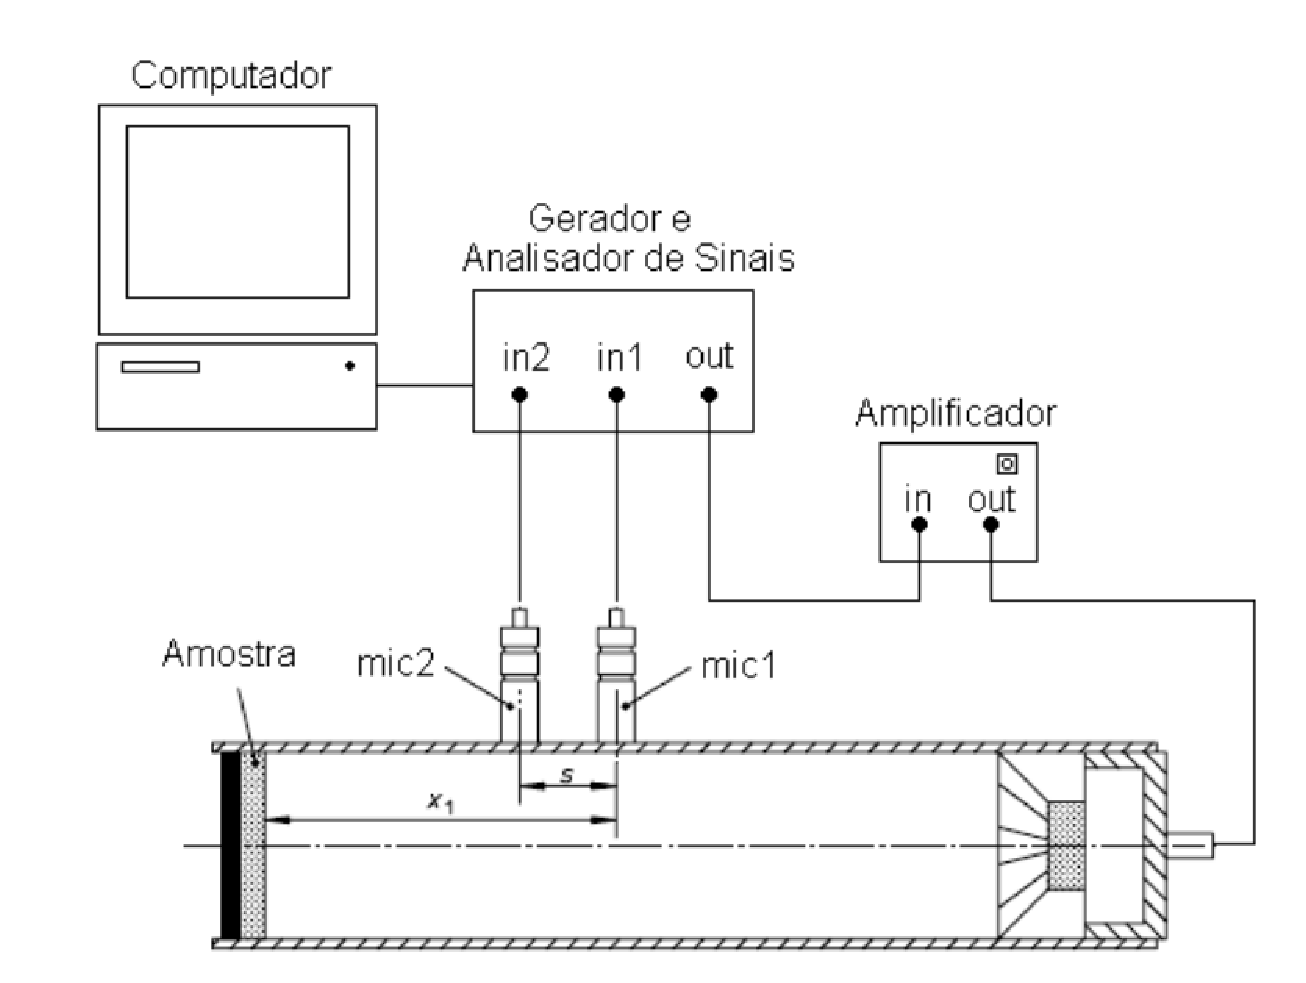
\includegraphics[scale=0.4]{figs/bancada.eps}
\caption{Tubo de impedância utilizado para a determinação dos coeficientes de absorção sonora das amostras.}
\label{fig.experimento}
\end{figure}

Para o processamento digital e aplicação dos cálculos das informações obtidas, foi desenvolvido um script do MATLAB. Segue o mesmo:
\lstinputlisting{processamento_duto.m}

\chapter{Resultados}\label{resultados}

\section{Coeficiente de Absorção}

Ao analisar o gráfico \ref{figura_1} é possível observar a variação coerente do coeficiente de absorção sonora, crescendo para as altas frequências e ficando abaixo do valor de 1, ou seja, $100\%$ de absorção. Também é possível observar os 3 tamanhos de espessuras diferentes, esse fato, somando a outros fatores, faz com que os coeficientes de absorção sejam ligeiramente diferentes.

\begin{figure}[h!]
    \centering
    %\hspace{-1.5cm}
    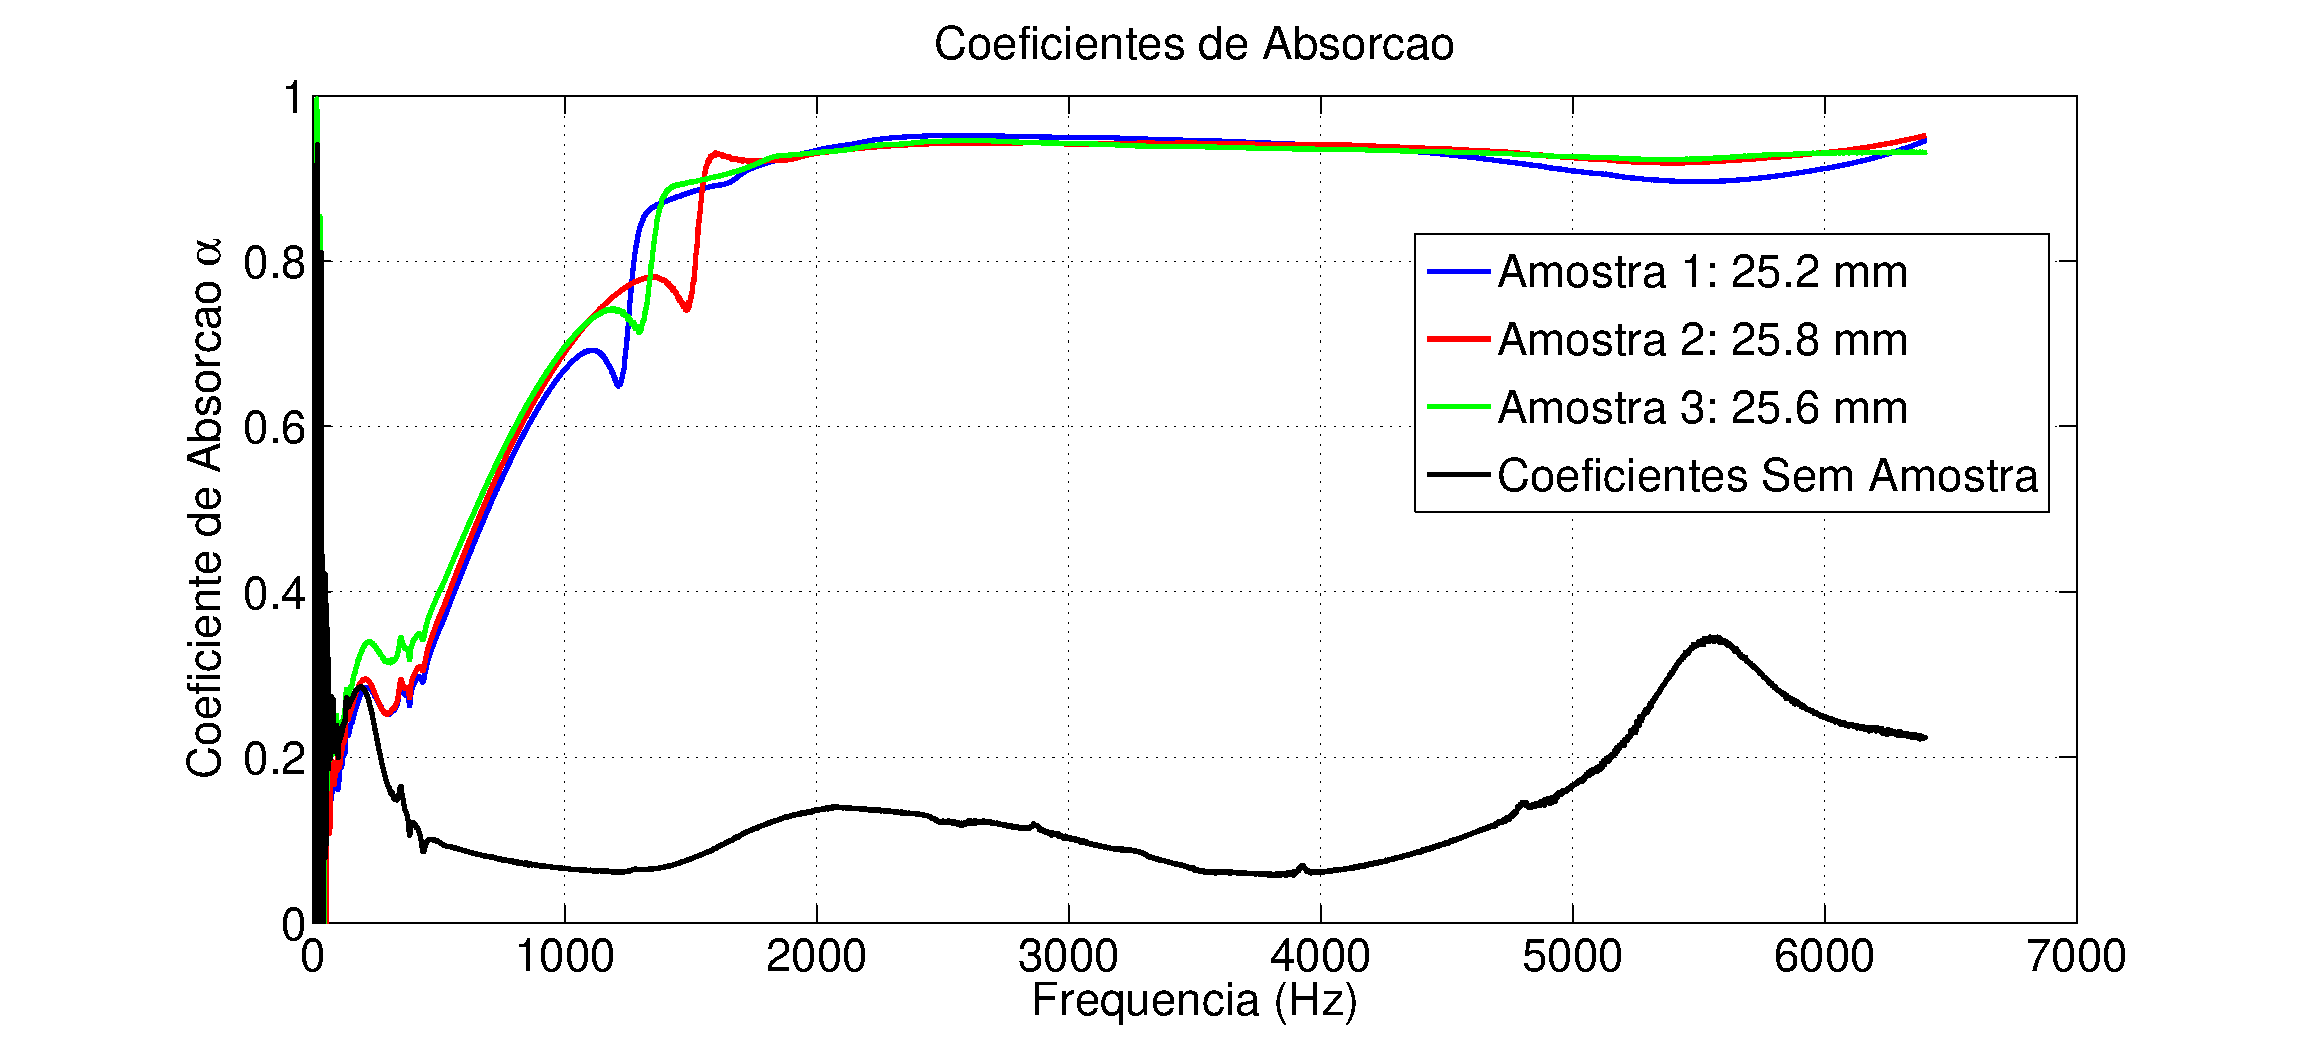
\includegraphics[width=1.1\textwidth]{tubo.eps}
    \caption{Coeficiente de absorção do material lâ de rocha. Fonte: autoria própria.}
    \label{figura_1}
\end{figure}


\chapter{Conclusões}\label{conclusoes}

Em vista do que foi apresentado, a realização dos ensaios no tubo de impedância originou resultados que constam de acordo com a teoria vigente visto que o coeficiente de absorção do material aumenta ao longo da frequência até num nível máximo 1 (100\% de absorção), e esse fato se repete para as 3 tipos de amostras consolidando um claro comportamento da absorção do material poroso.